\documentclass[tikz,border=8pt]{standalone}
% Shared look for every TikZ diagram. Load with % Shared look for every TikZ diagram. Load with % Shared look for every TikZ diagram. Load with \input{../../tools/tikz-style.tex}
\usepackage[T1]{fontenc}
\usepackage{lmodern}
\renewcommand{\sfdefault}{lmr}  % diagrams use the same serif as the text
\usetikzlibrary{arrows.meta, positioning, shapes.geometric, calc, fit, backgrounds}
\definecolor{cblue}{HTML}{4C78A8}
\definecolor{corange}{HTML}{F58518}
\definecolor{cgreen}{HTML}{54A24B}
\definecolor{cred}{HTML}{E45756}
\definecolor{cpurple}{HTML}{B279A2}
\definecolor{cgrey}{HTML}{6B6B6B}
\tikzset{
  every picture/.style={font=\sffamily, line width=1.2pt},
  box/.style={draw=#1, fill=#1!12, rounded corners=4pt, align=center, inner sep=7pt, minimum height=1.1cm},
  box/.default=cgrey,
  arrow/.style={-{Stealth[length=3mm]}, draw=cgrey, line width=1.4pt},
  title/.style={font=\sffamily\bfseries\Large},
  note/.style={font=\sffamily\small, text=cgrey, align=center},
}
\AtBeginDocument{\hyphenpenalty=10000 \exhyphenpenalty=10000}

\usepackage[T1]{fontenc}
\usepackage{lmodern}
\renewcommand{\sfdefault}{lmr}  % diagrams use the same serif as the text
\usetikzlibrary{arrows.meta, positioning, shapes.geometric, calc, fit, backgrounds}
\definecolor{cblue}{HTML}{4C78A8}
\definecolor{corange}{HTML}{F58518}
\definecolor{cgreen}{HTML}{54A24B}
\definecolor{cred}{HTML}{E45756}
\definecolor{cpurple}{HTML}{B279A2}
\definecolor{cgrey}{HTML}{6B6B6B}
\tikzset{
  every picture/.style={font=\sffamily, line width=1.2pt},
  box/.style={draw=#1, fill=#1!12, rounded corners=4pt, align=center, inner sep=7pt, minimum height=1.1cm},
  box/.default=cgrey,
  arrow/.style={-{Stealth[length=3mm]}, draw=cgrey, line width=1.4pt},
  title/.style={font=\sffamily\bfseries\Large},
  note/.style={font=\sffamily\small, text=cgrey, align=center},
}
\AtBeginDocument{\hyphenpenalty=10000 \exhyphenpenalty=10000}

\usepackage[T1]{fontenc}
\usepackage{lmodern}
\renewcommand{\sfdefault}{lmr}  % diagrams use the same serif as the text
\usetikzlibrary{arrows.meta, positioning, shapes.geometric, calc, fit, backgrounds}
\definecolor{cblue}{HTML}{4C78A8}
\definecolor{corange}{HTML}{F58518}
\definecolor{cgreen}{HTML}{54A24B}
\definecolor{cred}{HTML}{E45756}
\definecolor{cpurple}{HTML}{B279A2}
\definecolor{cgrey}{HTML}{6B6B6B}
\tikzset{
  every picture/.style={font=\sffamily, line width=1.2pt},
  box/.style={draw=#1, fill=#1!12, rounded corners=4pt, align=center, inner sep=7pt, minimum height=1.1cm},
  box/.default=cgrey,
  arrow/.style={-{Stealth[length=3mm]}, draw=cgrey, line width=1.4pt},
  title/.style={font=\sffamily\bfseries\Large},
  note/.style={font=\sffamily\small, text=cgrey, align=center},
}
\AtBeginDocument{\hyphenpenalty=10000 \exhyphenpenalty=10000}

\begin{document}
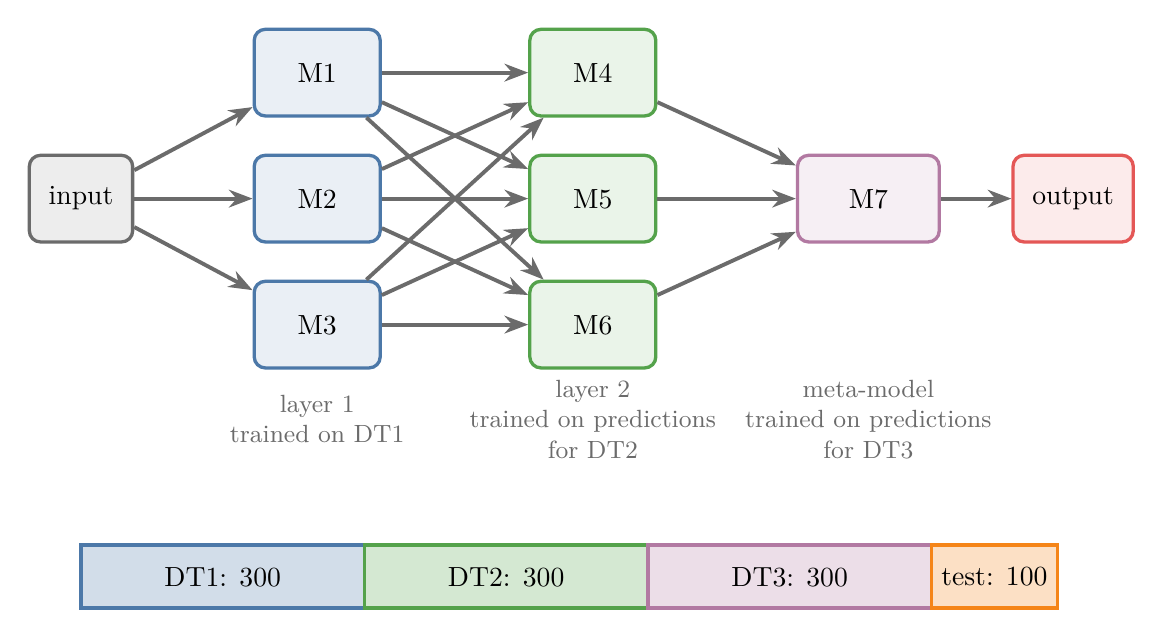
\begin{tikzpicture}[m/.style={box=cblue, minimum width=1.6cm}, n/.style={box=cgreen, minimum width=1.6cm},
  k/.style={box=cpurple, minimum width=1.8cm}]
  \node[box=cgrey] (x) at (0,0) {input};
  \foreach \i/\y in {1/1.6,2/0,3/-1.6} {\node[m] (a\i) at (3,\y) {M\i}; \draw[arrow] (x) -- (a\i);}
  \foreach \i/\y in {4/1.6,5/0,6/-1.6} {\node[n] (b\i) at (6.5,\y) {M\i};}
  \foreach \i in {1,2,3} {\foreach \j in {4,5,6} {\draw[arrow] (a\i) -- (b\j);}}
  \node[k] (meta) at (10,0) {M7};
  \foreach \j in {4,5,6} {\draw[arrow] (b\j) -- (meta);}
  \node[box=cred] (y) at (12.6,0) {output};
  \draw[arrow] (meta) -- (y);
  \node[note] at (3,-2.8) {layer 1\\trained on DT1};
  \node[note] at (6.5,-2.8) {layer 2\\trained on predictions\\for DT2};
  \node[note] at (10,-2.8) {meta-model\\trained on predictions\\for DT3};
  % the split
  \begin{scope}[yshift=-5.2cm]
  \fill[cblue!25, draw=cblue] (0,0) rectangle (3.6,0.8); \node at (1.8,0.4) {DT1: 300};
  \fill[cgreen!25, draw=cgreen] (3.6,0) rectangle (7.2,0.8); \node at (5.4,0.4) {DT2: 300};
  \fill[cpurple!25, draw=cpurple] (7.2,0) rectangle (10.8,0.8); \node at (9,0.4) {DT3: 300};
  \fill[corange!25, draw=corange] (10.8,0) rectangle (12.4,0.8); \node at (11.6,0.4) {test: 100};
  \end{scope}
\end{tikzpicture}
\end{document}
